\documentclass[11pt,letterpaper]{article}
\usepackage[utf8]{inputenc}
\usepackage[T1]{fontenc}
\usepackage{mathptmx}
\usepackage[letterpaper,left=1.25in,right=1.25in,top=1.2in,bottom=1.2in,headheight=14pt]{geometry}
\usepackage{microtype}
\usepackage{amsmath,amssymb,amsthm,mathtools,bm}
\usepackage{graphicx,booktabs,array,multirow,float}
\usepackage{xcolor}
\usepackage{enumitem}
\usepackage[labelfont=bf,labelsep=colon,font=small,skip=4pt]{caption}
\usepackage{subcaption}
\usepackage{fancyhdr}
\usepackage{titlesec}
\usepackage{listings}
\usepackage{tikz}
\usetikzlibrary{arrows.meta,positioning,calc}
\usepackage[authoryear,round]{natbib}
\definecolor{linkcol}{HTML}{2B3A8F}
\usepackage[colorlinks=true,linkcolor=linkcol,citecolor=linkcol,urlcolor=linkcol]{hyperref}
\usepackage[capitalise,noabbrev]{cleveref}

\pagestyle{fancy}\fancyhf{}
\lhead{\small Technical report.}
\cfoot{\small\thepage}
\renewcommand{\headrulewidth}{0.5pt}
\setlength{\parskip}{4pt plus 1pt}\setlength{\parindent}{0pt}
\titleformat{\section}{\large\bfseries}{\thesection}{0.8em}{}
\titleformat{\subsection}{\normalsize\bfseries}{\thesubsection}{0.8em}{}
\titleformat{\subsubsection}{\normalsize\bfseries\itshape}{\thesubsubsection}{0.8em}{}
\titlespacing*{\section}{0pt}{16pt}{6pt}\titlespacing*{\subsection}{0pt}{12pt}{4pt}
\setlist{itemsep=1pt,topsep=3pt}
\setlength{\emergencystretch}{2em}

\theoremstyle{definition}
\newtheorem{definition}{Definition}
\theoremstyle{remark}
\newtheorem{remark}{Remark}

\lstset{basicstyle=\ttfamily\small,breaklines=true,frame=single,framerule=0.3pt,
  xleftmargin=4pt,xrightmargin=4pt,columns=fullflexible,keepspaces=true,showstringspaces=false}

% title block: \reporttitle{title}{subtitle}{authors}{affiliation line}
\newcommand{\reporttitle}[4]{%
\begin{center}
{\LARGE\bfseries #1\\[4pt]
\Large #2\par}
\vspace{1.4em}
{\bfseries\color{linkcol}\large #3}\\[0.4em]
{\small #4}\par
\vspace{1.2em}
\end{center}}
\newcommand{\abstractblock}[1]{%
\begin{center}\textbf{Abstract}\end{center}
\vspace{-0.4em}
\begin{quote}\small #1\end{quote}
\vspace{0.4em}}

\begin{document}
\reporttitle{Mar\'ia: Farm Logistics on an Ontology}{Decision Support on Palantir Foundry and AIP}{Juan Fernando Casta\~no and team}{Palantir Build Challenge}

\abstractblock{Farm decisions depend on data that sits in different places: sensor readings, field records, schedules and guidance documents. A language model asked to advise on them directly has nothing to anchor its answers to. Mar\'ia is a decision-support application that models the farm as an ontology in Palantir Foundry, with entities, their relationships and the sensor time series attached to them, and places Palantir's Artificial Intelligence Platform (AIP) on top of that model. The model ranks what needs attention first and drafts a protocol for each item, with reference to FAO guidance so that a reviewer can check the recommendation against a recognised source. The application was built for the Palantir Build Challenge. This report describes its design and the reasoning behind it. It reports no performance figures, because none were measured.}

\section{Introduction}
Running a farm is a logistics problem as much as an agronomic one. Someone has to decide which field, animal or piece of equipment needs attention first, what to do about it, and whether that action is consistent with accepted practice. The inputs are scattered across sensors, spreadsheets and documents, and the person deciding is usually short of time.

A large language model can read and summarise this kind of material, but it is fluent without being grounded: it can produce a plausible recommendation that corresponds to nothing on the farm. We therefore ask one question. \textbf{Can a language model be made useful for farm operations by restricting it to a structured model of the farm and to a published source of guidance?}

\textbf{What we built.} Mar\'ia represents the farm as a set of typed objects with links between them, connects the sensor time series to those objects, and lets AIP work on the objects instead of on raw documents. It produces a ranked list of items that need attention and, for each, a draft protocol with reference to FAO guidance.

\textbf{Contributions.} The components are standard Foundry and AIP features. What we contribute is how they are combined:
\begin{enumerate}
\item an ontology of the farm in which the application, the analytics and the language model share one set of objects;
\item a triage step that runs on those objects, so a ranking can be traced to the data behind it;
\item a protocol-drafting step anchored to FAO guidance, so that every recommendation has an external point of reference.
\end{enumerate}

\section{Design}\label{sec:design}
\Cref{fig:flow} shows the flow of information.
\begin{figure}[t]\centering
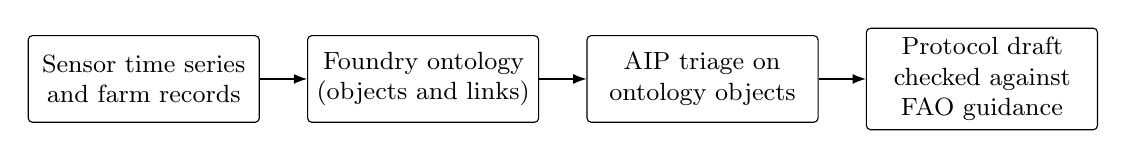
\begin{tikzpicture}[>=Latex,node distance=6mm,s/.style={draw,rounded corners=1.5pt,minimum height=11mm,text width=2.7cm,align=center,font=\small}]
 \node[s] (a) {Sensor time series and farm records};
 \node[s,right=of a] (b) {Foundry ontology (objects and links)};
 \node[s,right=of b] (c) {AIP triage on ontology objects};
 \node[s,right=of c] (d) {Protocol draft checked against FAO guidance};
 \draw[->] (a)--(b); \draw[->] (b)--(c); \draw[->] (c)--(d);
\end{tikzpicture}
\caption{Information flow in Mar\'ia.}\label{fig:flow}
\end{figure}

\textbf{Ontology.} In Foundry, an ontology maps datasets to objects with properties and links \citep{palantirdocs}. Modelling the farm this way means a reading, the thing it was taken from and the work planned for that thing are connected, and a question about one can reach the others.

\textbf{Triage.} AIP is given the objects, not the underlying files. It ranks what needs attention and explains the ranking in terms of the properties it used. A reviewer can open the object and see the same values.

\textbf{Protocols.} For each item the model drafts a recommended action and relates it to FAO guidance \citep{faogap}. The draft is a proposal, and a person decides whether to act on it.

\section{Discussion}\label{sec:discussion}
Putting the model on top of an ontology narrows what it can talk about to what the farm actually contains, and anchoring protocols to a published source gives the reviewer something concrete to check. Both measures reduce, but do not remove, the chance of a confident wrong answer.

\textbf{What this report does not establish.} We did not measure the accuracy of the ranking, the quality of the drafted protocols, or the time saved. The application was demonstrated in the challenge walkthrough; it was not evaluated against a baseline or deployed on a working farm. The report does not describe object types, data volumes or model configuration beyond what is stated above.

\textbf{Next steps.} The first step is an evaluation: have an agronomist rank a set of historical situations and compare the ranking with the model's. After that, protocol drafts should be scored against the guidance they cite.

\section*{Code and data availability}
The walkthrough of the application is at \url{https://youtu.be/ssvYMJInNas}. The application lives in a Foundry workspace and is not part of this repository, which holds this report and its source.

\bibliographystyle{plainnat}
\bibliography{references}
\end{document}
